\section{Introdução à pneumática}

\begin{frame}{Introdução}
\begin{block}{O que é?}
	\begin{itemize}
		\item A \textbf{pneumática} é o ramo da engenharia que \textbf{estuda} e \textbf{faz uso }de \textbf{gases comprimidos}.
	\end{itemize}
\end{block}

\vspace{0.2cm}

\centering
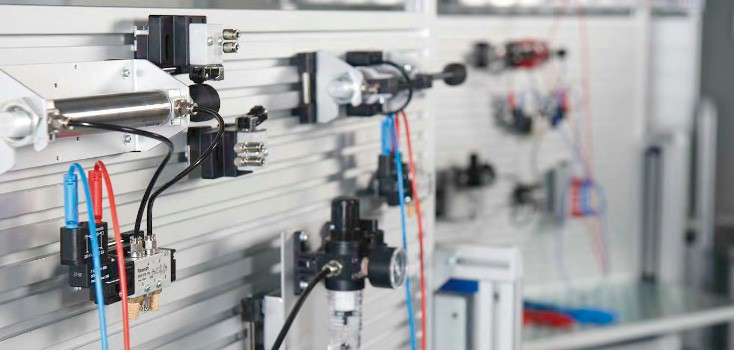
\includegraphics[width=0.9\linewidth]{Figuras/Ch11/fig1}

\end{frame}


\begin{frame}{Introdução}
\begin{block}{Compressor}
	\begin{itemize}
		\item Na indústria é utilizado principalmente \textbf{ar atmosférico} comprimido por um \textbf{compressor}.
	\end{itemize}
\end{block}

\centering
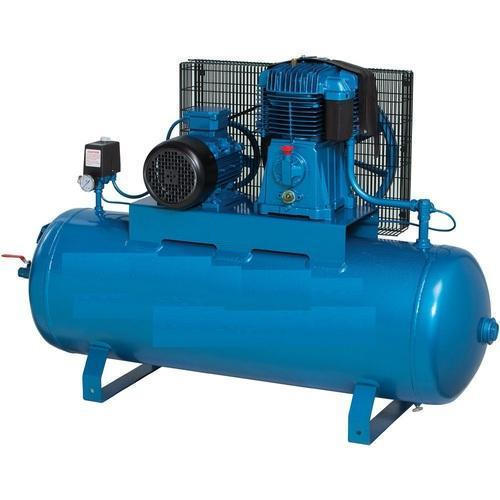
\includegraphics[width=0.5\linewidth]{Figuras/Ch11/fig2}

\end{frame}


\begin{frame}{Introdução}
	\begin{block}{Aplicações}
		\begin{itemize}
			\item Um compressor gera o ar comprimido que será utilizado em uma variedade de aplicações, como \textbf{cilindros}, \textbf{motores} ou \textbf{ferramentas pneumáticas.}
		\end{itemize}
	\end{block}
	
	\begin{minipage}{0.45\linewidth}
		\centering
		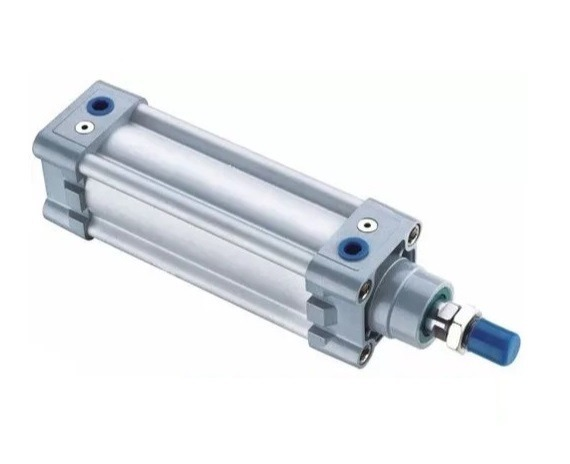
\includegraphics[width=1\linewidth]{Figuras/Ch11/fig2n1}
	\end{minipage}
	\hfill
	\begin{minipage}{0.45\linewidth}
		\centering
		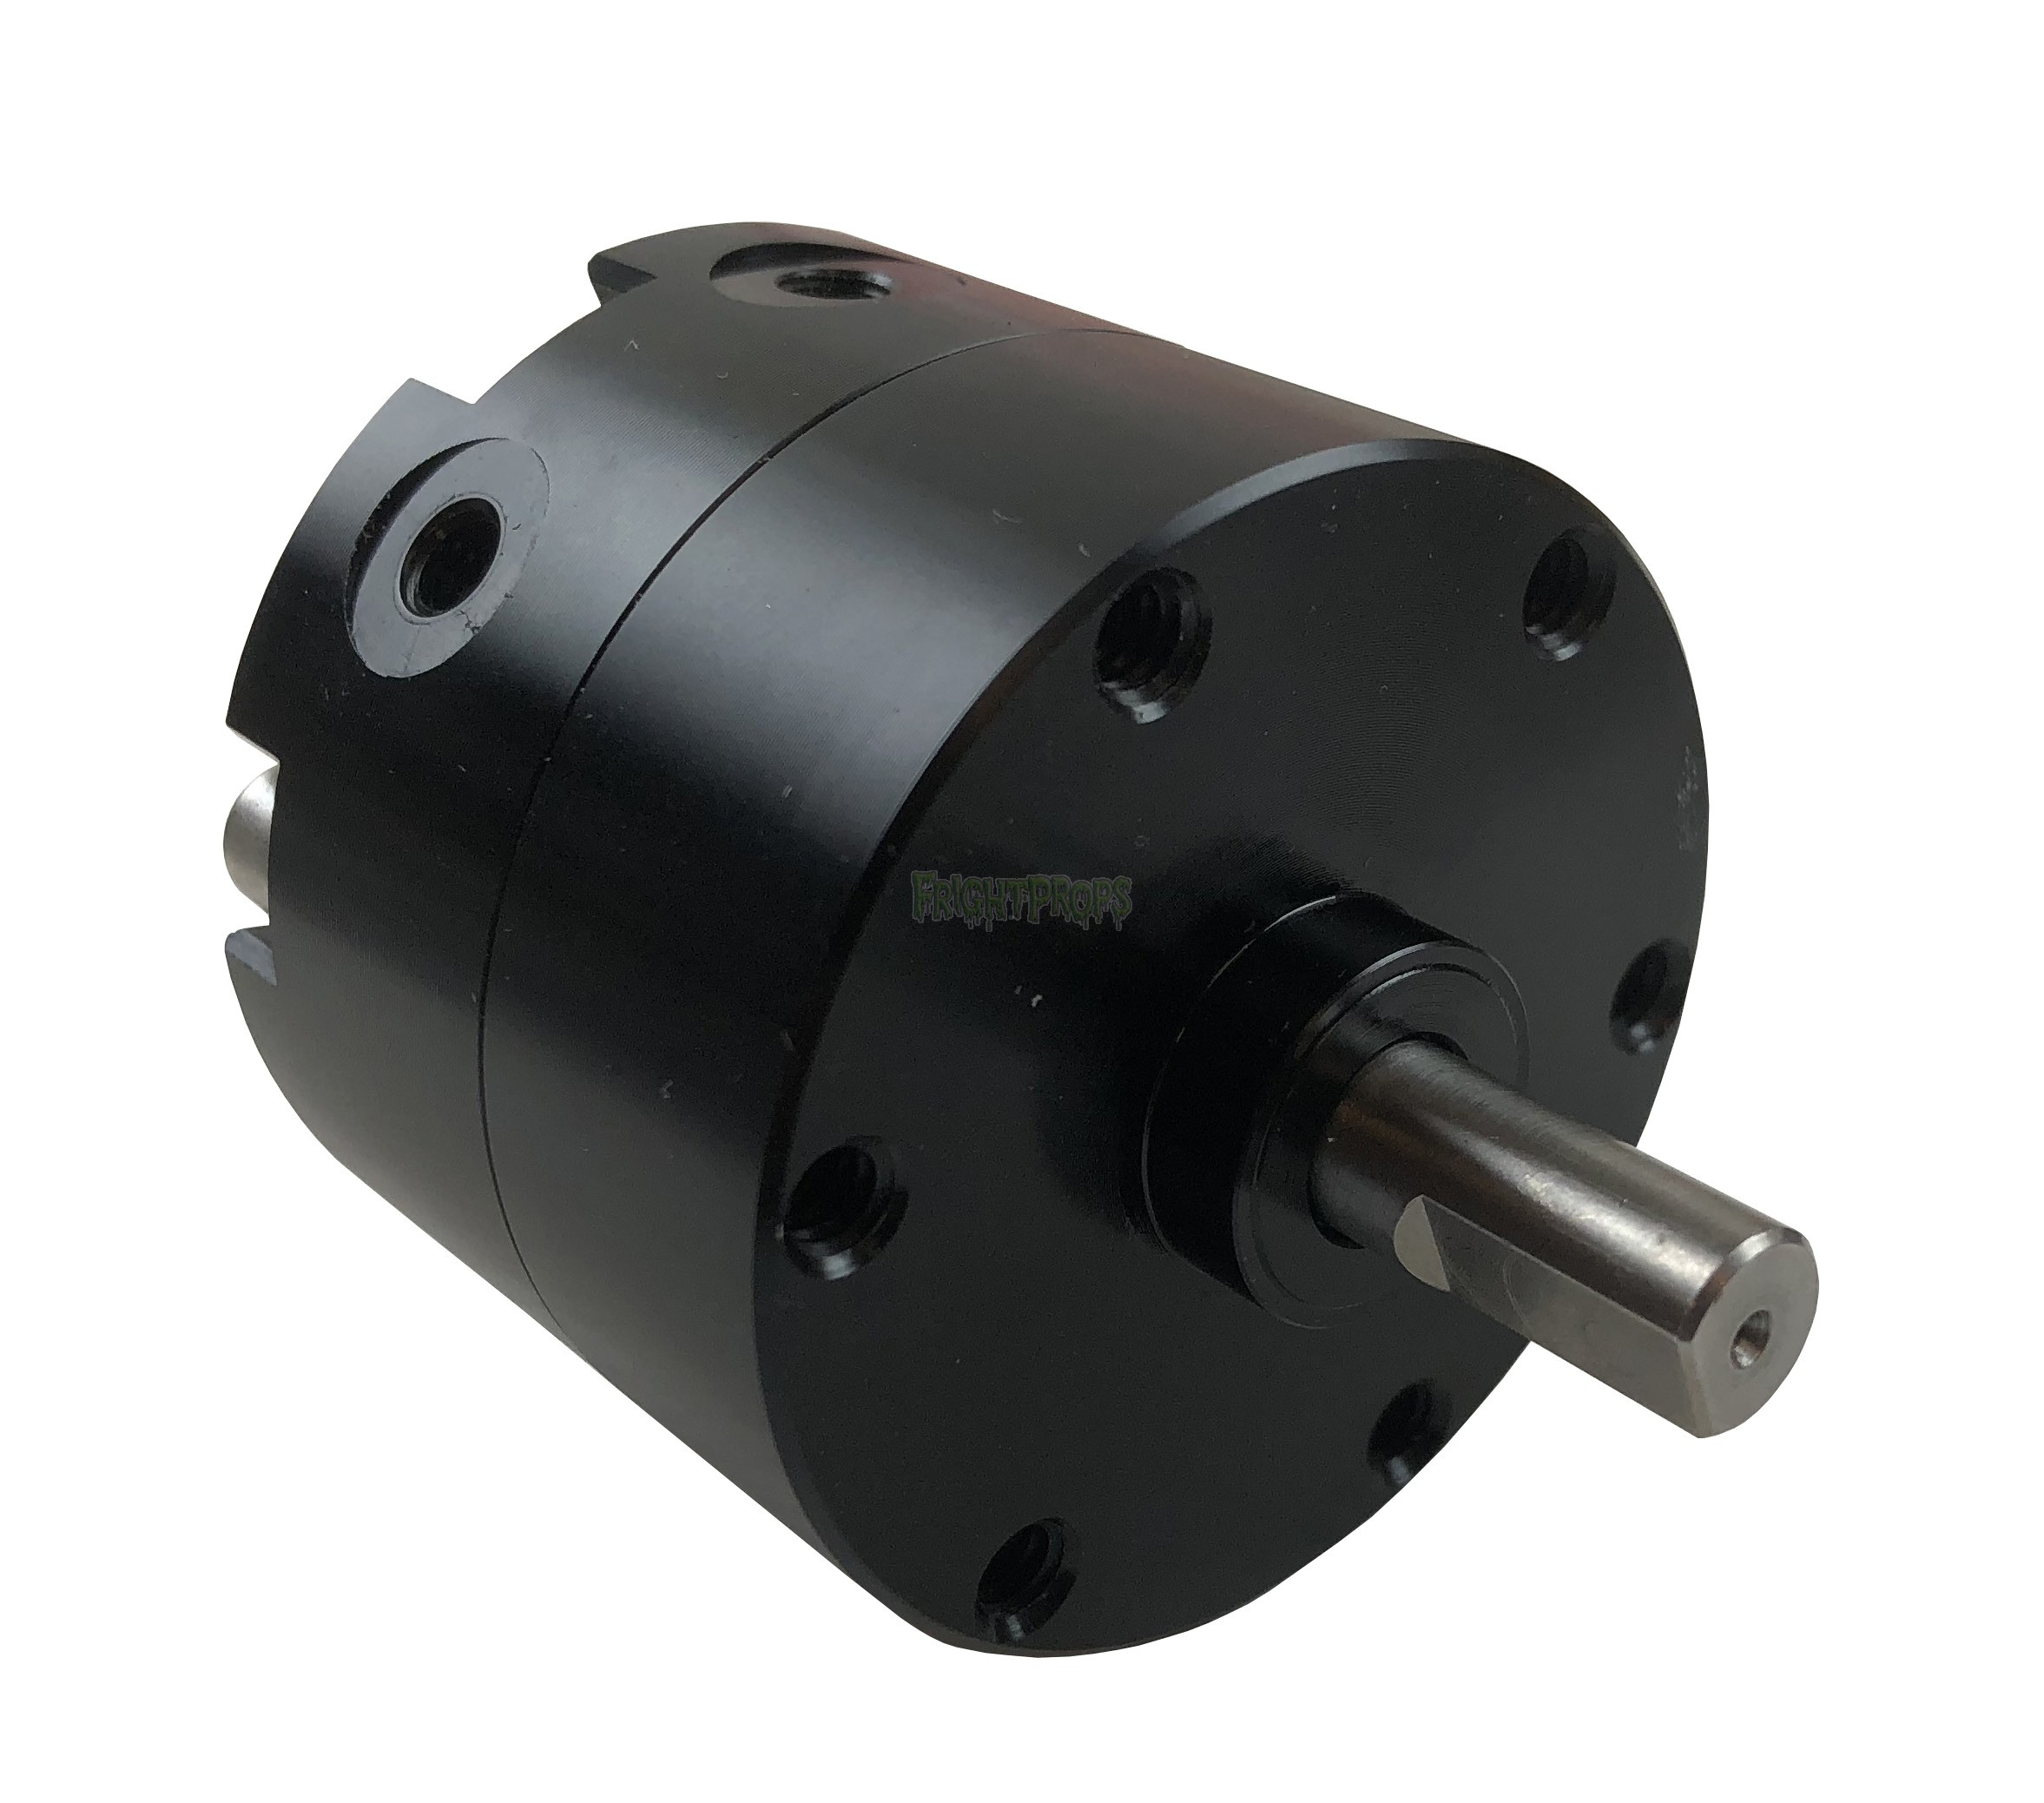
\includegraphics[width=1\linewidth]{Figuras/Ch11/fig2n2}
	\end{minipage}
	
\end{frame}


\begin{frame}{Introdução}
\begin{block}{Controle}
	\begin{itemize}
		\item Um sistema com pneumática pode ser controlado por \textbf{válvulas manuais ou solenoide.}
	\end{itemize}
\end{block}

\begin{minipage}{0.45\linewidth}
	\centering
	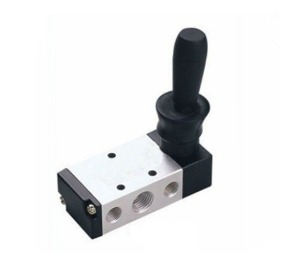
\includegraphics[width=1\linewidth]{Figuras/Ch11/fig3}
	
	Válvula pneumática manual
\end{minipage}
\hfill
\begin{minipage}{0.45\linewidth}
	\centering
	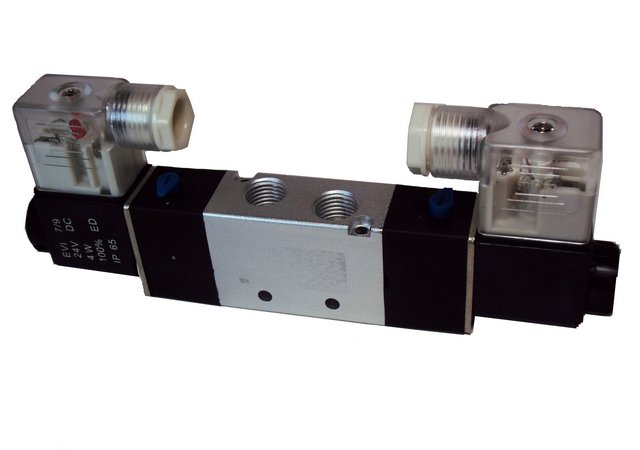
\includegraphics[width=1\linewidth]{Figuras/Ch11/fig4}
	
	Válvula pneumática solenoide
\end{minipage}
\end{frame}


\begin{frame}{Introdução}
	\begin{block}{Vantagens}
		\begin{itemize}
			\item Normalmente é uma opção \textbf{mais barata, mais flexível e segura} do que uma alternativa elétrica ou hidráulica.
			\item Robusta, pois não é tão sensível a \textbf{vibrações} e \textbf{golpes}, podendo trabalhar também em ambientes mais hostis.
			\item Fácil de implementar.
			\item Simples de operar.
			\item Segura, pois trabalha com pressões moderadas.
		\end{itemize}
	\end{block}
\end{frame}


\begin{frame}{Introdução}
	\begin{block}{Limitações}
		\begin{itemize}
			\item O ar comprimido precisa de \textbf{boa preparação} para ser utilizado.
			\item Os componentes pneumáticos não são capazes de trabalhar com \textbf{grandes forças}, devido à limitação de pressão dos sistemas.
			\item O movimento em baixa velocidade é difícil.
			\item Por conta da compressibilidade do ar, velocidades uniformes e paradas intermediárias são difíceis.
		\end{itemize}
	\end{block}
\end{frame}


\begin{frame}{Introdução}
	\begin{block}{Utilização}
		\begin{itemize}
			\item A pneumática é usada em uma variedade enorme de aplicações e indústrias: indústrias de embalagens, de alimentos e bebidas, automotiva, entre outras.
		\end{itemize}
	\end{block}

\centering
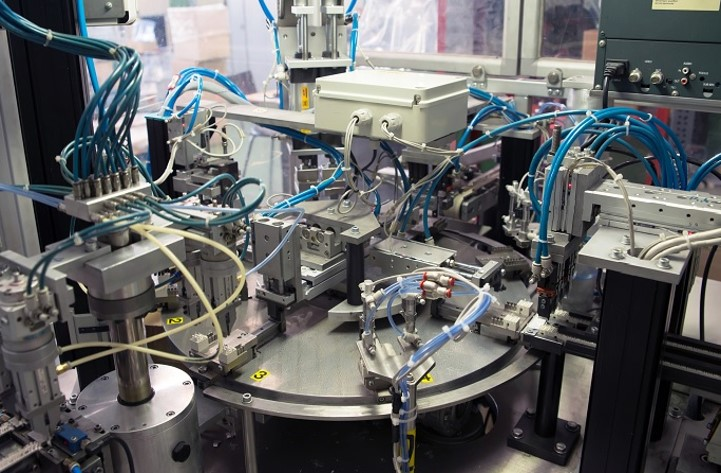
\includegraphics[width=0.7\linewidth]{Figuras/Ch11/fig5}
\end{frame}


\begin{frame}{Pressão}
\begin{block}{Introdução}
	\begin{itemize}
		\item Para controlarmos um sistema pneumático é necessário ter ar comprimido, isto é, ar que teve seu volume reduzido e, por isso, agora está \textbf{pressurizado}.
		\item Mas \textbf{o que é pressão?}
	\end{itemize}
\end{block}
\end{frame}


\begin{frame}{Pressão}
\begin{block}{O que é?}
	\begin{itemize}
		\item A \textbf{pressão} é definida como sendo a razão entre a força e a área: \[ P=\dfrac{\vec{F}}{A} \]
	\end{itemize}
\end{block}

\vspace{0.5cm}

\centering
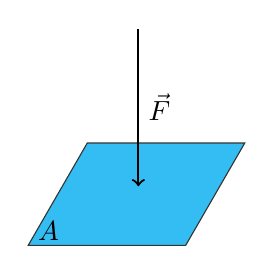
\begin{tikzpicture}
	\filldraw[fill=cyan!80,draw=black!80!white] (0,0) node[right,yshift=5pt] {$ A $} -- (60:1.5) -- ++(2,0) -- +(-120:1.5) -- cycle;
	\draw[<-,thick] (30:1.5) ++(0.1,0) -- +(0,2) node[right,midway] {$ \vec{F} $};
\end{tikzpicture}
\end{frame}


\begin{frame}{Tipos de pressão}
	\begin{block}{Pressão atmosférica}
		\begin{itemize}
			\item A atmosfera é cheia de gases, e a pressão que exercem é chamada \textbf{pressão atmosférica}.
			\item A pressão atmosférica varia com a altitude.
		\end{itemize}
	\end{block}

\centering
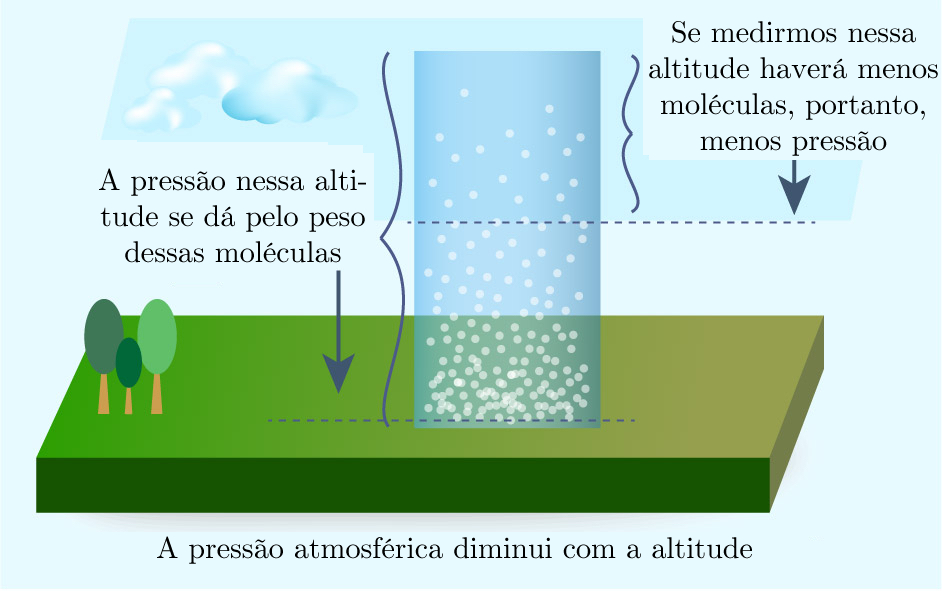
\includegraphics[width=0.7\linewidth]{Figuras/Ch11/fig6n1}
\end{frame}


\begin{frame}{Tipos de pressão}
	\begin{block}{Pressão atmosférica}
		\begin{itemize}
			\item Em 1643 Evangelista Torricelli quantificou a pressão atmosférica utilizando um tubo cheio de mercúrio.
		\end{itemize}
	\end{block}
	
	\vspace{0.5cm}
	
	\centering
	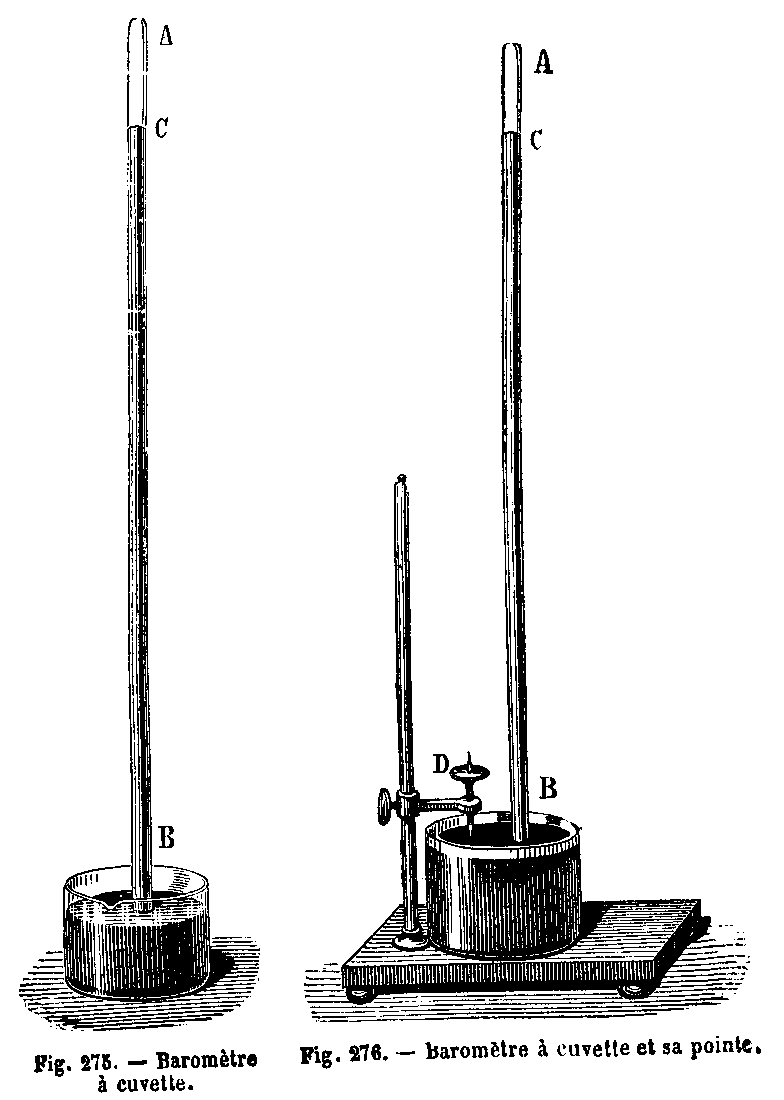
\includegraphics[height=0.6\textheight]{Figuras/Ch11/fig6n2}
\end{frame}


\begin{frame}{Tipos de pressão}
	\begin{block}{Pressão atmosférica}
		\begin{itemize}
			\item O experimento de Torricelli consistiu em preencher (em 75\%) um tubo com mercúrio e então virá-lo dentro de um recipiente maior, que sofreria influência da atmosfera.
			\item Como a coluna de mercúrio só sofre ação da coluna de ar da atmosfera, \textbf{suas pressões devem se igualar}.
			\item O resultado de Torricelli é que a pressão atmosférica ao nível do mar equivale a \num{760} milímetros de mercúrio, isto é, \SI{760}{\mmHg}.
		\end{itemize}
	\end{block}
	
	\centering
	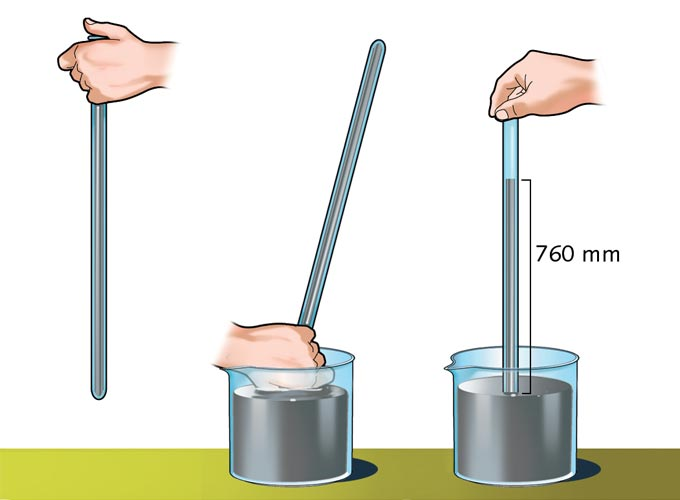
\includegraphics[height=0.4\textheight]{Figuras/Ch11/fig7}
\end{frame}


\begin{frame}{Tipos de pressão}
	\begin{block}{Vácuo absoluto}
		\begin{itemize}
			\item É de onde começamos a medir.
		\end{itemize}
	\end{block}
	
	\vspace{3.5cm}
	
	\centering
	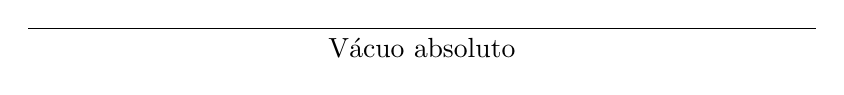
\begin{tikzpicture}
		\draw (0,0) -- node[below, midway] {Vácuo absoluto} (10,0);
	\end{tikzpicture}
\end{frame}


\begin{frame}{Tipos de pressão}
	\begin{block}{Pressão manométrica}
		\begin{itemize}
			\item É a pressão relativa à atmosférica.
		\end{itemize}
	\end{block}
	
	\vspace{0.5cm}
	
	\centering
	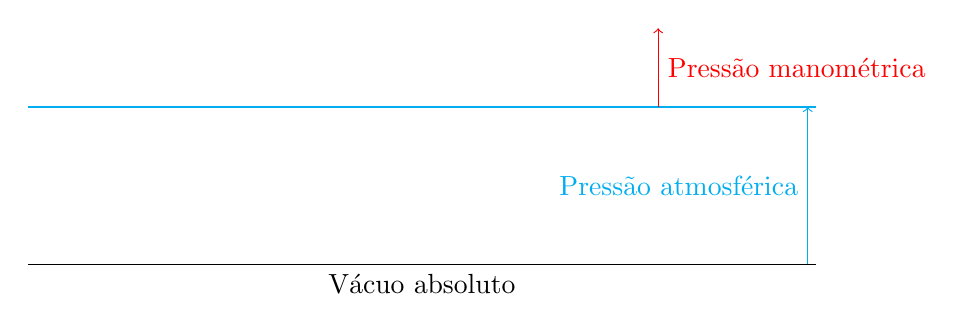
\begin{tikzpicture}
	\draw (0,0) -- node[below, midway] {Vácuo absoluto} (10,0);
	\draw[cyan] (0,2) -- +(10,0);
	\draw[->,cyan] (9.9,0) -- node[left, midway] {Pressão atmosférica} +(0,2);
	\draw[->,red] (8,2) -- node[midway,right] {Pressão manométrica} +(0,1);
	\end{tikzpicture}
\end{frame}


\begin{frame}{Tipos de pressão}
	\begin{block}{Pressão de vácuo}
		\begin{itemize}
			\item É a pressão negativa em relação à atmosférica.
		\end{itemize}
	\end{block}
	
	\vspace{0.5cm}
	
	\centering
	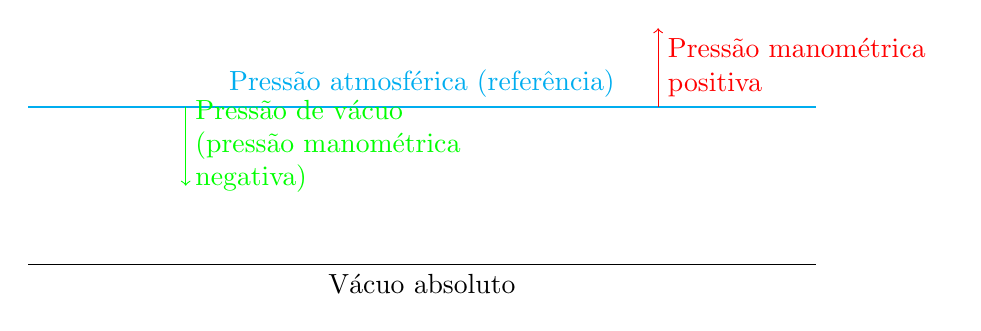
\begin{tikzpicture}
	\draw (0,0) -- node[below, midway] {Vácuo absoluto} (10,0);
	\draw[cyan] (0,2) -- node[above, midway] {Pressão atmosférica (referência)} +(10,0);
%	\draw[->,cyan] (9.9,0) -- node[left, midway] {Pressão atmosférica} +(0,2);
	\draw[->,red] (8,2) -- node[midway,right,text width=3.5cm] {Pressão manométrica positiva} +(0,1);
	\draw[->,green] (2,2) -- node[midway,right, text width=4cm] {Pressão de vácuo (pressão manométrica negativa)} +(0,-1);
	\end{tikzpicture}
\end{frame}


\begin{frame}{Tipos de pressão}
	\begin{block}{Pressão absoluta}
		\begin{itemize}
			\item É a pressão total medida a partir do vácuo.
		\end{itemize}
	\end{block}
	
	\vspace{0.5cm}
	
	\centering
	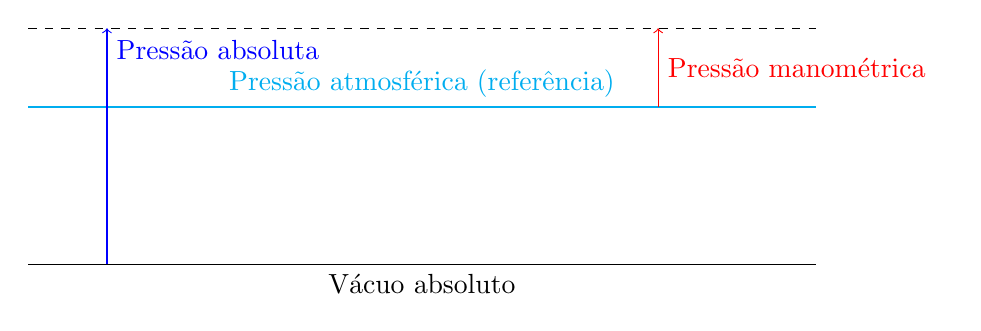
\begin{tikzpicture}
	\draw (0,0) -- node[below, midway] {Vácuo absoluto} (10,0);
	\draw[cyan] (0,2) -- node[above, midway] {Pressão atmosférica (referência)} +(10,0);
	%	\draw[->,cyan] (9.9,0) -- node[left, midway] {Pressão atmosférica} +(0,2);
	\draw[->,red] (8,2) -- node[midway,right,text width=3.5cm] {Pressão manométrica} +(0,1);
%	\draw[->,green] (2,2) -- node[midway,right, text width=4cm] {Pressão de vácuo (pressão manométrica negativa)} +(0,-1);
	\draw[blue,->] (1,0) -- +(0,3) node[right, very near end, yshift=3pt] {Pressão absoluta};
	\draw[dashed] (0,3) -- +(10,0); 
	\end{tikzpicture}
\end{frame}


\begin{frame}{Tipos de pressão}
	\centering
	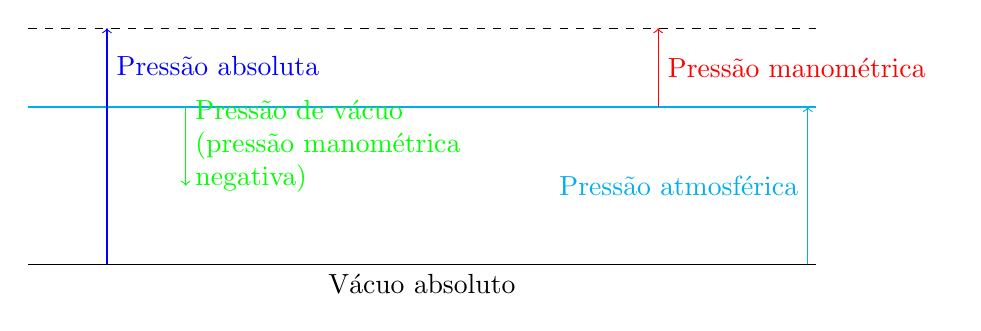
\begin{tikzpicture}
	\draw (0,0) -- node[below, midway] {Vácuo absoluto} (10,0);
	\draw[cyan] (0,2) -- +(10,0);
		\draw[->,cyan] (9.9,0) -- node[left, midway] {Pressão atmosférica} +(0,2);
	\draw[->,red] (8,2) -- node[midway,right,text width=3.5cm] {Pressão manométrica} +(0,1);
		\draw[->,green] (2,2) -- node[midway,right, text width=4cm] {Pressão de vácuo (pressão manométrica negativa)} +(0,-1);
	\draw[blue,->] (1,0) -- +(0,3) node[right, very near end, yshift=-3pt] {Pressão absoluta};
	\draw[dashed] (0,3) -- +(10,0); 
	\end{tikzpicture}
\end{frame}


\begin{frame}{Unidades de pressão}
\begin{block}{}
	A pressão pode ser medida usando diversas \textbf{unidades}, entre elas:
	\begin{itemize}
		\item $ \si{\psip}$ $(=\si{\psid}) $ - Sistema inglês
		\item $ \si{\atm} $ - Pressão atmosférica ao nível do mar (aprox.)
		\item $ \si{\kgfp} $ - Unidade técnica
		\item $ \si{\pascal}$ $(=\si{\newton\per\meter\squared}) $ - Sistema internacional (SI)
		\item $ \si{\barp}$ $(=\SI{10000}{\pascal}=10^5\,\si{\pascal}) $
		\item $ \si{\mca} $
		\item $ \si{\mmHg} $
	\end{itemize}
\end{block}
\end{frame}


\begin{frame}{Unidades de pressão}
	\centering
	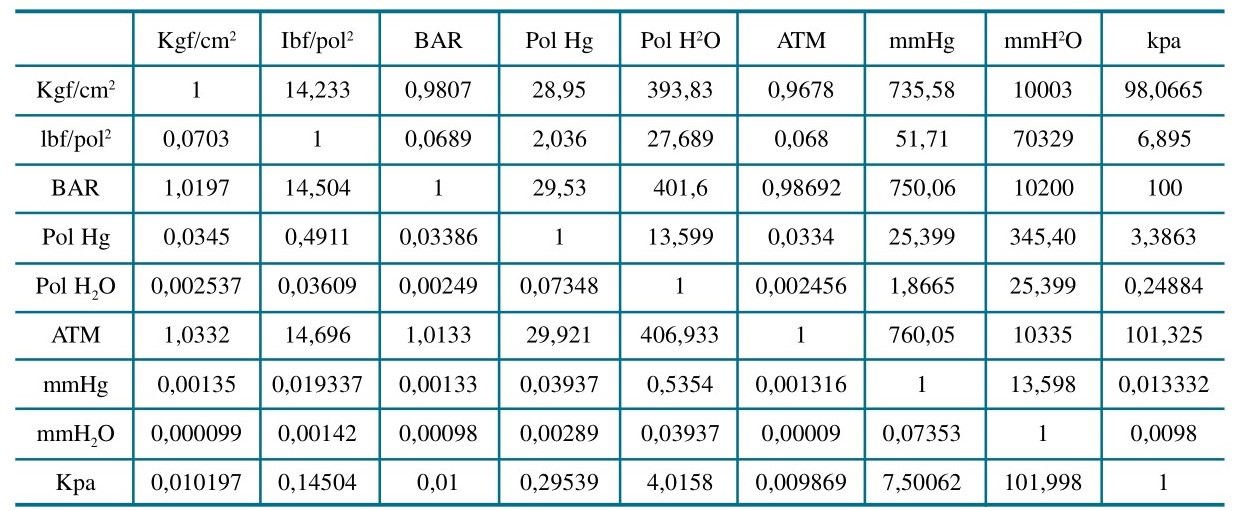
\includegraphics[width=1\linewidth]{Figuras/Ch11/fig8}
\end{frame}


\begin{frame}{Ar}
\begin{block}{Introdução}
	Sendo o ar nosso instrumento de estudo, cabe saber algumas de suas \textbf{propriedades}, como:
	\begin{itemize}
		\item Compressibilidade
		\item Elasticidade
		\item Difusibilidade
		\item Expansibilidade
	\end{itemize}
\end{block}
\end{frame}


\begin{frame}{Ar - Propriedades}
	\begin{block}{Compressibilidade}
		\begin{itemize}
			\item O ar permite reduzir o seu volume quando sujeito à ação de uma força exterior.
		\end{itemize}
	\end{block}
\centering
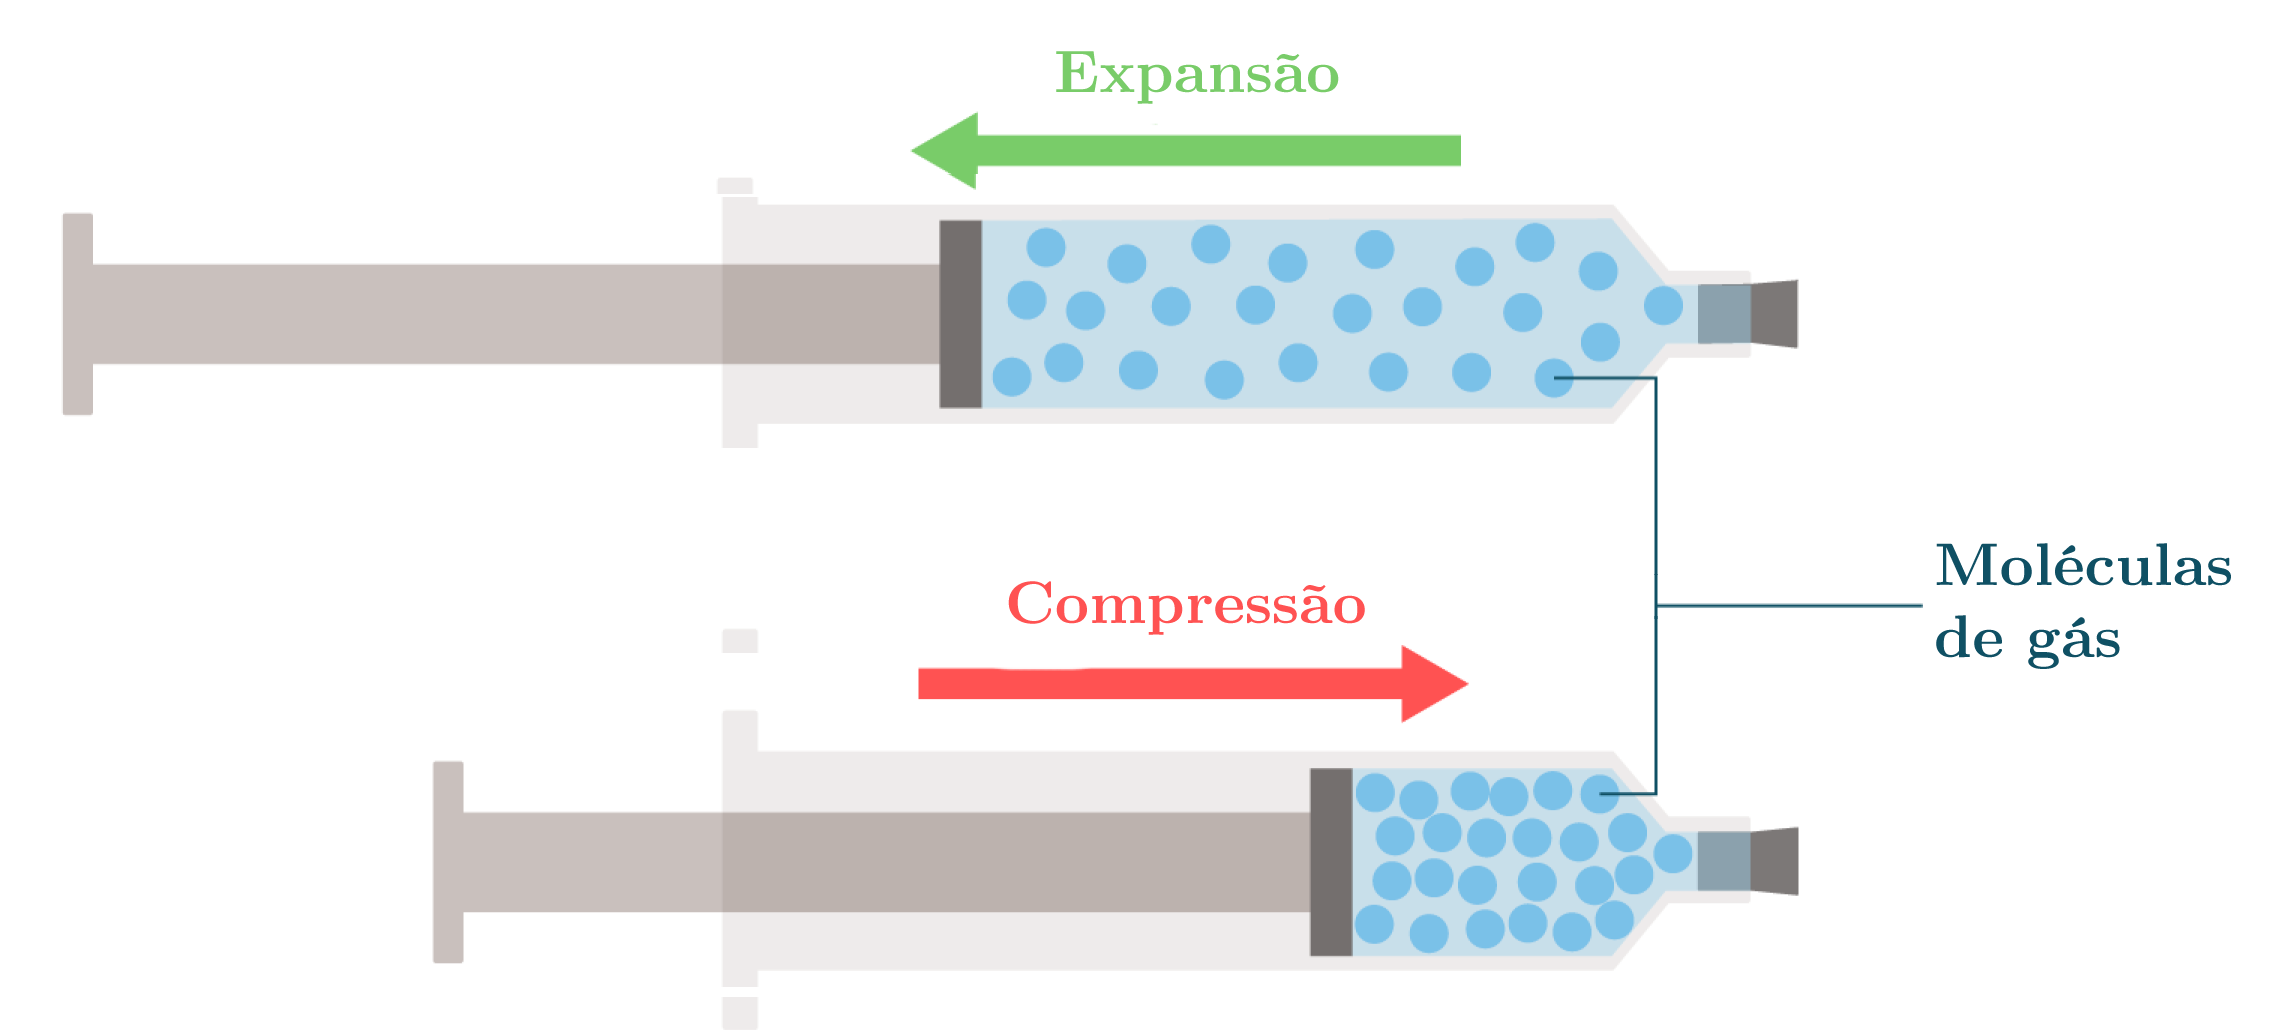
\includegraphics[width=1\linewidth]{Figuras/Ch11/fig9}
\end{frame}


\begin{frame}{Ar - Propriedades}
	\begin{block}{Elasticidade}
		\begin{itemize}
			\item O ar volta ao seu volume inicial uma vez extinto o efeito (força) responsável pela redução do volume.
		\end{itemize}
	\end{block}
\centering
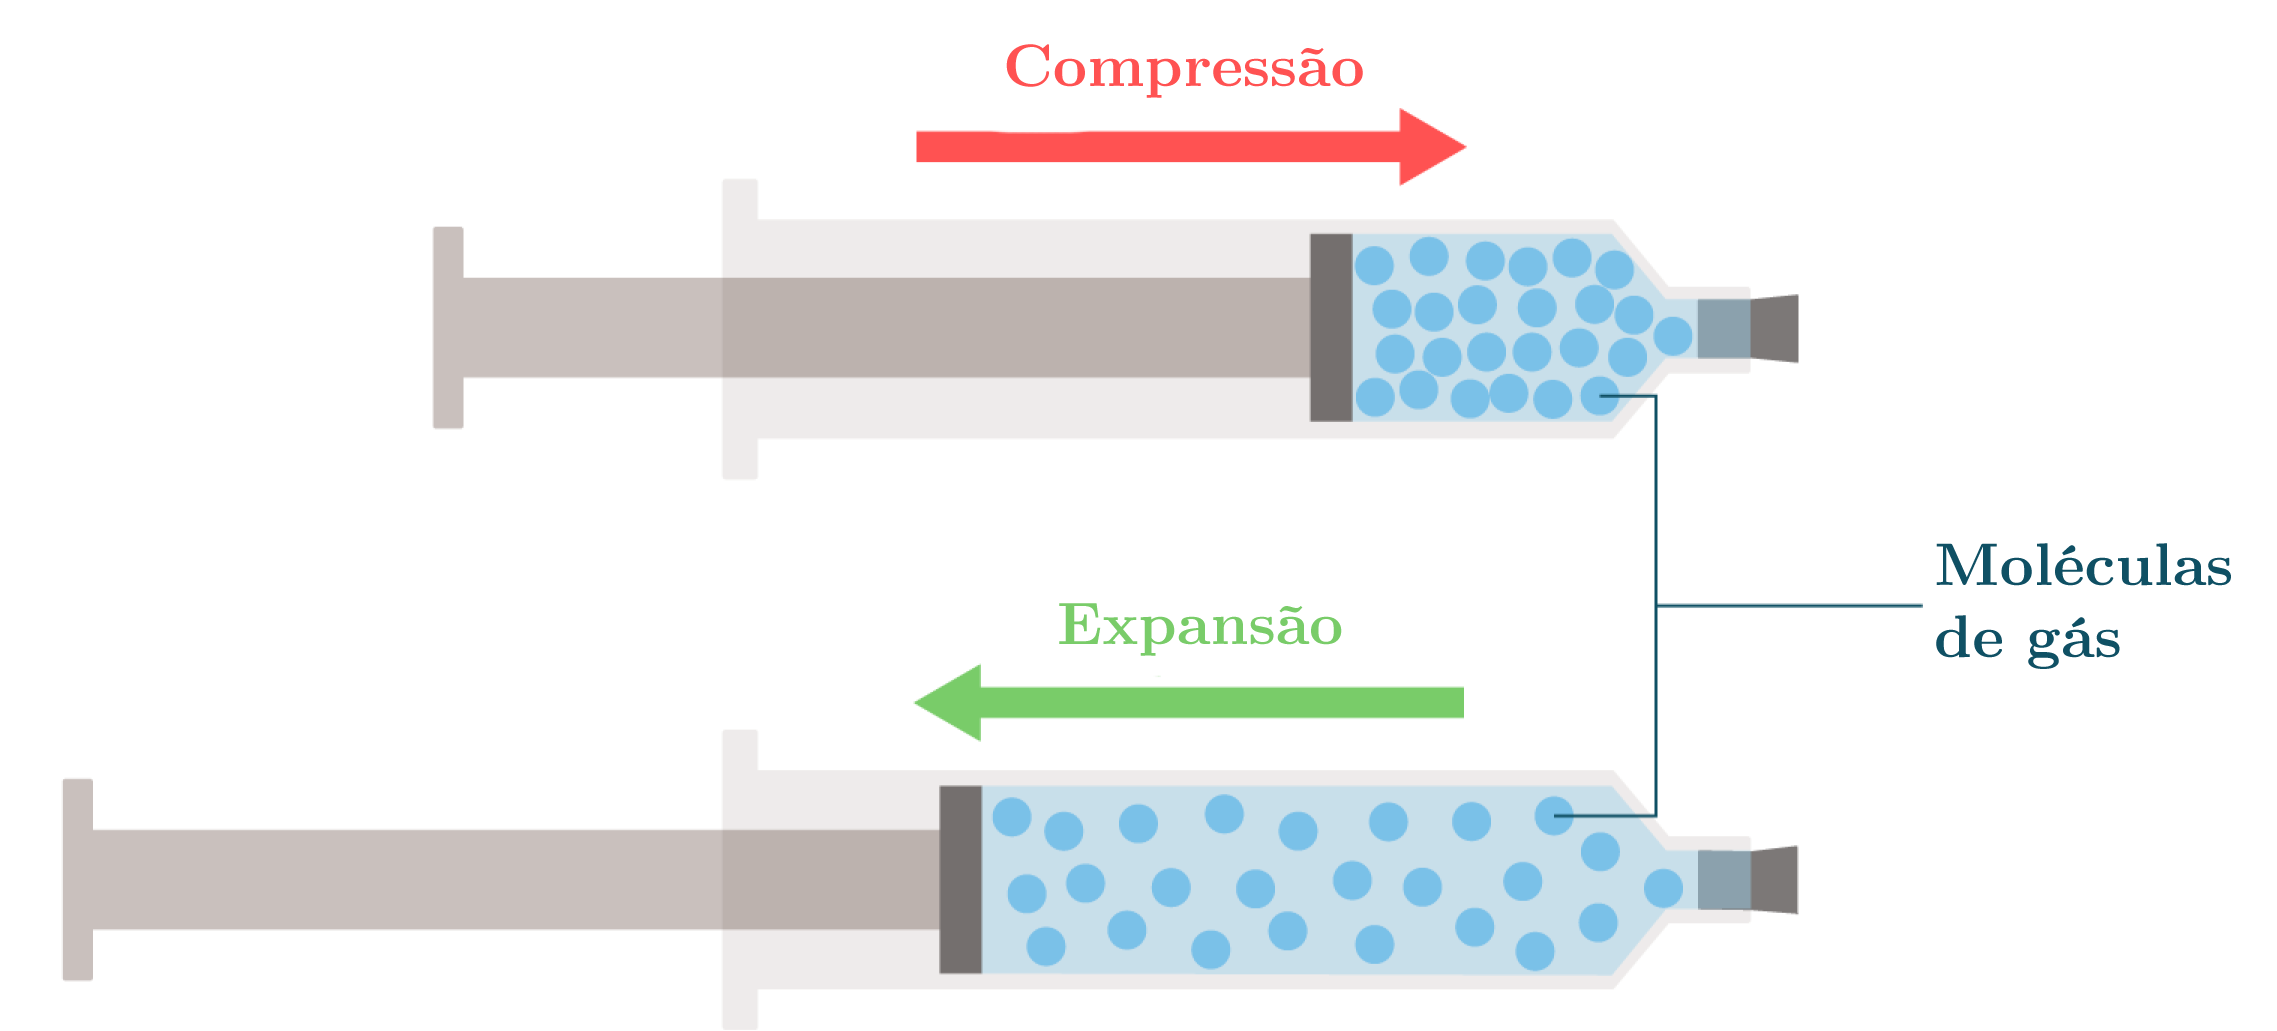
\includegraphics[width=1\linewidth]{Figuras/Ch11/fig10}
\end{frame}


\begin{frame}{Ar - Propriedades}
	\begin{block}{Difusibilidade}
		\begin{itemize}
			\item O ar se mistura homogeneamente com qualquer meio gasoso que não esteja saturado.
		\end{itemize}
	\end{block}
\vspace{0.5cm}

\centering
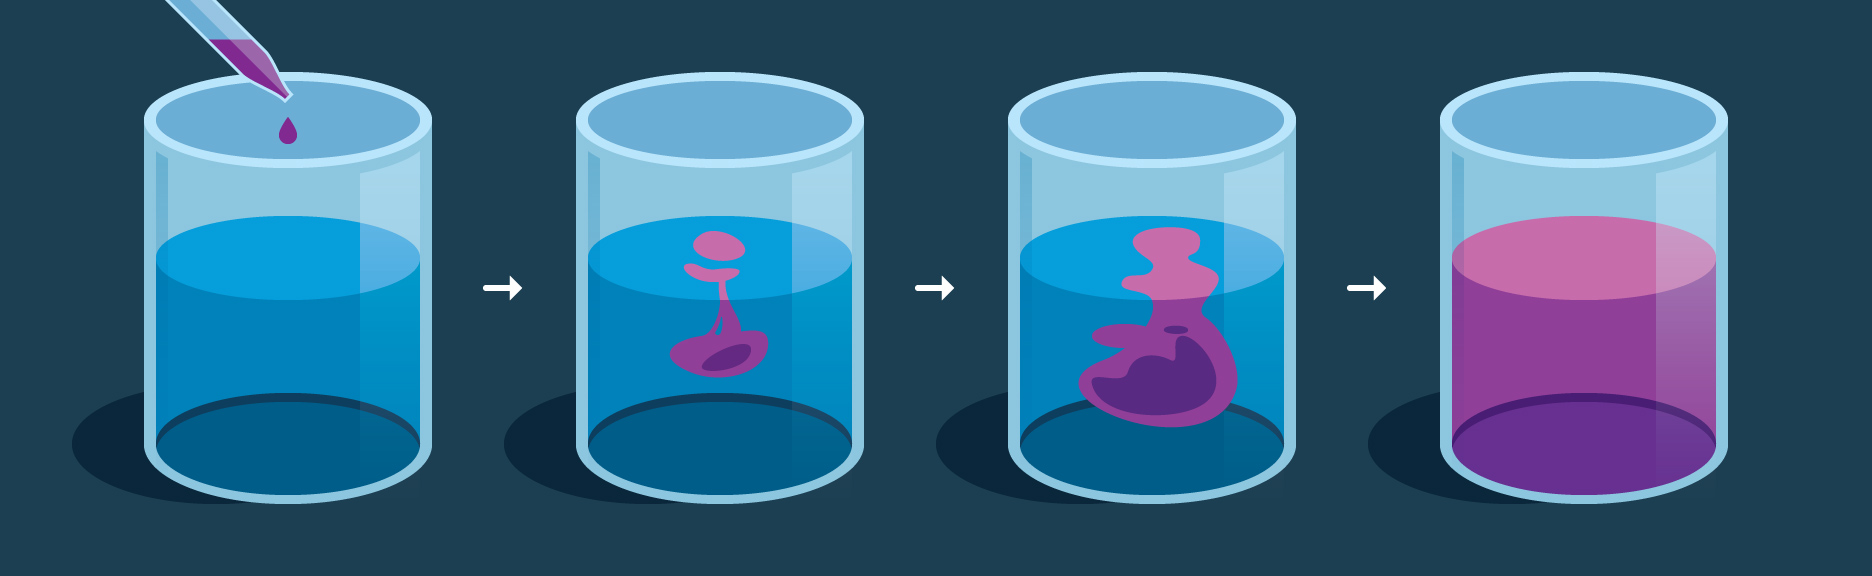
\includegraphics[width=1\linewidth]{Figuras/Ch11/fig11}
\end{frame}


\begin{frame}{Ar - Propriedades}
	\begin{block}{Expansibilidade}
		\begin{itemize}
			\item O ar ocupa totalmente o volume de qualquer recipiente, adquirindo o seu formato.
		\end{itemize}
	\end{block}
\vspace{0.5cm}

\centering
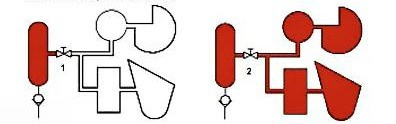
\includegraphics[width=1\linewidth]{Figuras/Ch11/fig12}
\end{frame}


\frame{
	\frametitle{Exercícios}
	\begin{block}{}
		01. Sabendo que o ar gelado é mais denso do que o ar quente, quais propriedades do ar atuam em uma geladeira e em quais momentos?
		
		\vspace{0.5cm}
		
		02. Um manômetro (medidor de pressão) é instalado num tanque fechado e mostra \SI{-0.5}{\barp}. De qual pressão, entre as abordadas nessa aula, estamos tratando? O que você acha?
	\end{block}
}

\section*{Referências}
\frame{
	\frametitle{Referências e Exercícios Complementares}
	\begin{itemize}
		\item MELCONIAN, Sarkis. Sistemas Fluidomecânicos - Hidráulica e Pneumática, 1 ed. Érica, 2014.
	\end{itemize}
	%\centering{\alert{Página 546 - \textbf{Capítulo 6}}} \\
	%\centering{\alert{Lista de exercícios 01}}
}